\chapter{Steps in the analysis}

To apply the rule-of-thumb one should carry out the following five steps.
\dfastmi can perform steps 2 and 4 for you (except for the computation of $z_\text{mdd}$).

\begin{enumerate}
\item Characterize the measure to be evaluated using \dfastmi

\begin{itemize}
\item Determine the threshold discharge $Q_\text{thr}$ (at Lobith/Borgharen) at which the measure (indirectly) starts to influence the flow pattern in the main channel.

\item Determine the bankfull discharge $Q_\text{bf}$ (at Lobith/Borgharen) at which the measure is fully flooded (bankfull flow)
\end{itemize}

\item Define the discharge blocks (block 1 "low flow", block 3 "flood" and block 2 "transitional between low and flood flows") using

\begin{itemize}
\item \autoref{Tab7} for the Rhine branches
\item \autoref{Tab8} for the Meuse
\end{itemize}

\item Perform the (up to six) necessary hydrodynamic simulations

\item Compute the characteristic bed level change per grid point in the main channel

\begin{itemize}
\item maximum value \unitbrackets{m} at the end of the flood season

\begin{equation}
z_{b,1}(0) = \frac{z_{b,1,\text{eq}} (1-\sigma_1) \sigma_2 \sigma_3 + z_{b,2,\text{eq}} (1-\sigma_2) \sigma_3 + z_{b,3,\text{eq}} (1-\sigma_3)}{1 - \sigma_1 \sigma_2 \sigma_3}
\end{equation}

\item minimum value \unitbrackets{m} at the end of the low flow season

\begin{equation}
z_{b,2}(0) = \frac{z_{b,1,\text{eq}} (1-\sigma_1) + z_{b,2,\text{eq}} (1-\sigma_2) \sigma_3 \sigma_1 + z_{b,3,\text{eq}} (1-\sigma_3) \sigma_1}{1 - \sigma_1 \sigma_2 \sigma_3}
\end{equation}

\item transitional value \unitbrackets{m} at the end of the transition block before the flood period

\begin{equation}
z_{b,3}(0) = \frac{z_{b,1,\text{eq}} (1-\sigma_1) \sigma_2 + z_{b,2,\text{eq}} (1-\sigma_2) + z_{b,3,\text{eq}} (1-\sigma_3) \sigma_1 \sigma_2}{1 - \sigma_1 \sigma_2 \sigma_3}
\end{equation}

\item year-averaged value \unitbrackets{m}

\begin{equation}
z_{b,m} = T_1 z_{b,1}(0) + T_2 z_{b,2}(0) + T_3 z_{b,3}(0)
\end{equation}

\item the maximum dredging depth (ignoring any excess depth)

\begin{equation}
z_\text{mdd} = z_{b,1,\text{eq}} (1-\sigma_1) \sigma_2 \sigma_3 + z_{b,2,\text{eq}} (1-\sigma_2) \sigma_3 + z_{b,3,\text{eq}} (1-\sigma_3)
\end{equation}
\end{itemize}

\item{Visualize the characteristic bed level changes in a graph or on a map}

\end{enumerate}

\begin{table}
\caption{Definition of discharge blocks for the Rhine branches}
\label{Tab7}
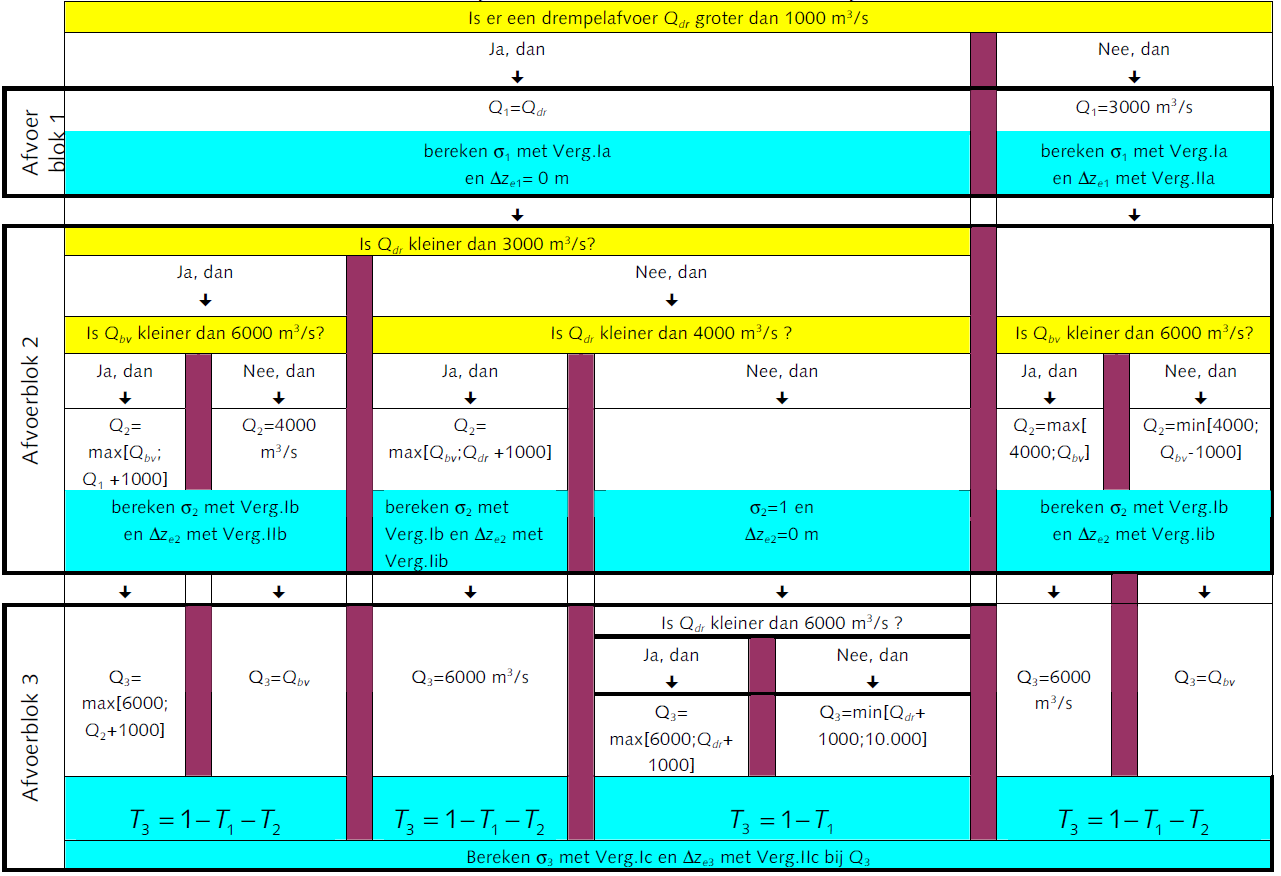
\includegraphics[width=\columnwidth]{figures/Tab7.png}
%
\begin{equation}
\sigma_1 = e^{-\frac{w_l}{2 B_n} T_1}
\end{equation}
with $T_1 = e^{\left ( \frac{800-Q_\text{bar}}{1280} \right )} - e^{\left ( \frac{800-Q_1}{1280} \right )}$ and $w_l$ from \autoref{Tab4RT} (with $Q_\text{bar} = 1500$ m\textsuperscript{3}/s for Nederrijn and Lek and $Q_\text{stuw} = 800$ m\textsuperscript{3}/s for the other branches)
%
\begin{equation}
\sigma_2 = e^{-\frac{w_h}{2 B_n} T_2}
\end{equation}
%
\begin{equation}
\sigma_3 = e^{-\frac{w_h}{2 B_n} T_3}
\end{equation}
with $T_2 = e^{\left ( \frac{800-Q_1}{1280} \right )} - e^{\left ( \frac{800-Q_2}{1280} \right )}$ and $w_h$ from \autoref{Tab4RT}.
%
\begin{equation}
\Delta z_{b,1,\text{eq}} = -h_o \frac{u_n - u_o}{u_o} \text{  for $Q_1$}
\end{equation}
%
\begin{equation}
\Delta z_{b,2,\text{eq}} = -h_o \frac{u_n - u_o}{u_o} \text{  for $Q_2$}
\end{equation}
%
\begin{equation}
\Delta z_{b,3,\text{eq}} = -h_o \frac{u_n - u_o}{u_o} \text{  for $Q_3$}
\end{equation}
based on reference water depths $h_o$ and velocities $u_o$ and modified velocities $u_n$ from the simulations.
\end{table}


\begin{table}
\caption{Definition of discharge blocks for the Meuse}
\label{Tab8}
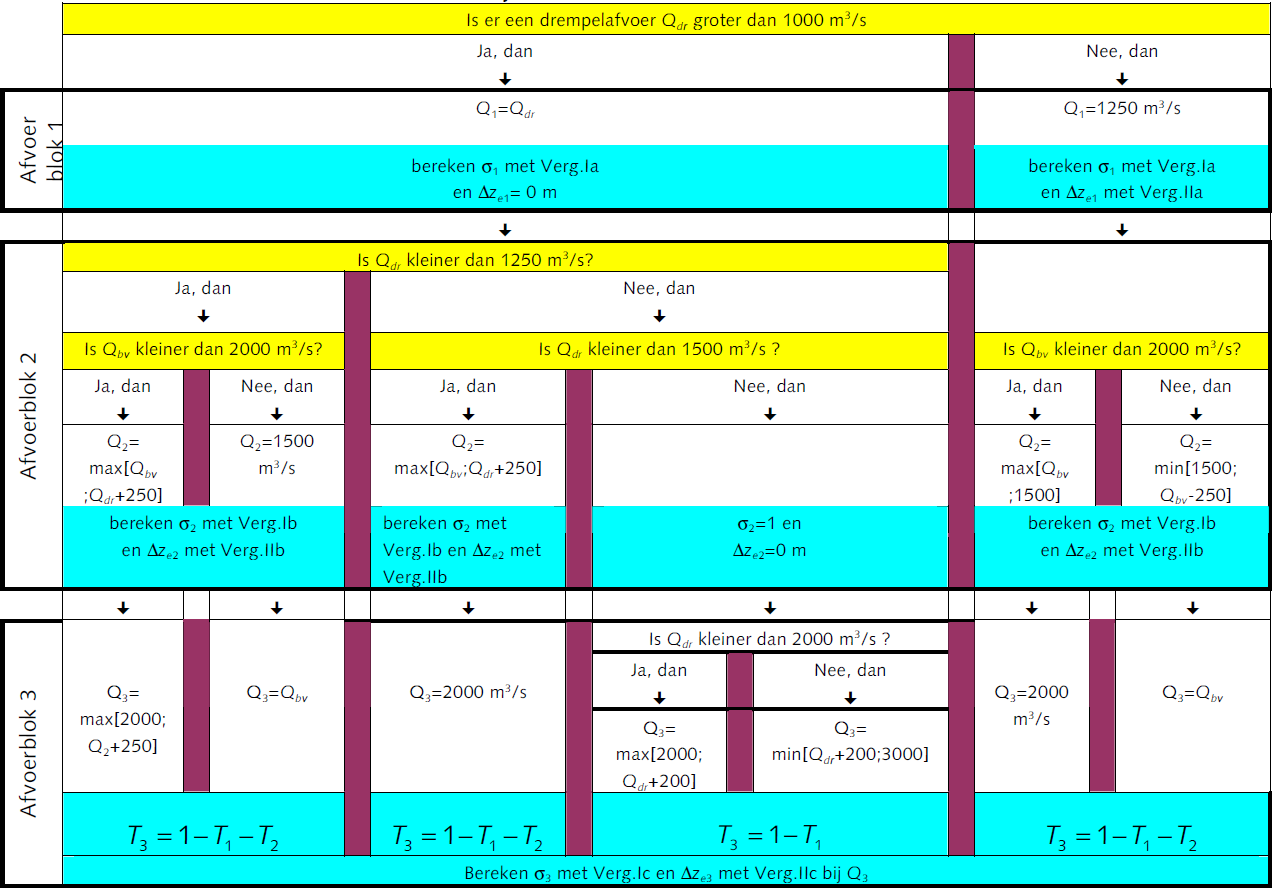
\includegraphics[width=\columnwidth]{figures/Tab8.png}
%
\begin{equation}
\sigma_1 = e^{-\frac{w_l}{2 B_n} T_1}
\end{equation}
with $T_1 = e^{\left ( - \frac{Q_\text{bar}}{300} \right )} - e^{\left ( - \frac{Q_1}{300} \right )}$; $Q_\text{bar} = 100$ m\textsuperscript{3}/s and $w_l$ from \autoref{Tab5}.
%
\begin{equation}
\sigma_2 = e^{-\frac{w_h}{2 B_n} T_2}
\end{equation}
%
\begin{equation}
\sigma_3 = e^{-\frac{w_h}{2 B_n} T_3} \text{ with $w_h$ from \autoref{Tab8}}
\end{equation}
 with $T_2 = e^{\left ( - \frac{Q_1}{300} \right )} - e^{\left ( - \frac{Q_2}{300} \right )}$ and $w_h$ from \autoref{Tab5}.
%
\begin{equation}
\Delta z_{b,1,\text{eq}} = -h_o \frac{u_n - u_o}{u_o} \text{  for $Q_1$}
\end{equation}
%
\begin{equation}
\Delta z_{b,2,\text{eq}} = -h_o \frac{u_n - u_o}{u_o} \text{  for $Q_2$}
\end{equation}
%
\begin{equation}
\Delta z_{b,3,\text{eq}} = -h_o \frac{u_n - u_o}{u_o} \text{  for $Q_3$}
\end{equation}
based on reference water depths $h_o$ and velocities $u_o$ and modified velocities $u_n$ from the simulations.

The premisses are: the flow in the main channel is well developed at $Q = 1000$ m\textsuperscript{3}/s, and at $Q = 2000$ m\textsuperscript{3}/s the flows in main channel and floodplain are both well developed.
\end{table}
